\documentclass[a4paper]{article}

\usepackage{amsfonts}
\usepackage{amssymb}
\usepackage{graphicx}
\usepackage{xcolor}
\usepackage{geometry}
\usepackage{titling}
\usepackage{caption}
\usepackage{algorithm}
\usepackage[noend]{algpseudocode}
\usepackage{listings}
\usepackage{xparse}
\usepackage{blindtext}
\usepackage{hyperref}
\hypersetup{
    colorlinks=true,
    linkcolor=blue,
    filecolor=magenta,      
    urlcolor=cyan,
    pdftitle={Overleaf Example},
    pdfpagemode=FullScreen,
    }

\NewDocumentCommand{\codeword}{v}{%
\texttt{\textcolor{red}{#1}}%
}
\lstdefinestyle{sharpc}{language=[Sharp]C, frame=lr, rulecolor=\color{blue!80!black}}

\geometry{
   left=25.4mm,
   right=25.4mm,
   top=25.4mm,
   bottom=25.4mm,
}
\setlength{\droptitle}{-27mm}

\begin{document}
\author{Shridhar Thorat: n10817239}
\title{Assignment 1: CAB301}
\maketitle
\tableofcontents
\setcounter{page}{0}

\section{Introduction}
The goal of this assignment was to design 3 Abstract Data types (ADTs) in a C\# environment. This report aims to design pseudocode algorithms for the three methods in \textit{Scheduler}, and implement them in C\#. As well as determining their theoretical efficiency and describing the effects during implementation. It will also include a test plan for the three ADT's designed.
\vspace{-0.5cm}
\section{Algorithm Design and Analysis}
For the simple purposes of this assignment and selection having a fairly simple implementation in C\#, \textit{Scheduler} implements the \textit{selection} sort algorithm for all three methods in a similar method to the pseudocode in page 98---100\hyperlink{section.4}{(Levitin, 2012)}. The Selection sort algorithm can be directly translated with some minor changes. These minor changes are due to C\# being the language of use and due to design choices for the \textit{Job}, \textit{JobCollection} and \textit{Scheduler} classes.
\\[6pt]
Each sorting algorithm uses a \textit{JobCollection} called \textit{Jobs} which is a property of a \textit{schedule}. \textit{Jobs} is an array of \textit{job} objects and has some \textit{capacity} and \textit{count}. If we consider that the collection is expressed as $Jobs[0,\ldots,capacity-1]$, then the number of jobs in the collection is expressed as $Jobs[0,\ldots,count-1]$. For the purposes of pseudocode and time efficiency, $count$ will be considered as $n$ and the worst case time efficiency function will be relative to it. This is because when sorting, null values can be ignored as they are `empty'. Therefore, the sorting algorithms need only iterate over the jobs in a collection --- hence the time efficiency is relative to $count$ rather than $capacity$.
\\[6pt]
Additionally, each algorithm used a method from the \textit{JobCollection} class called \codeword{ToArray()} which creates an independent \textit{IJob} array so as to prevent editing the original, unsorted array of jobs. This method requires first instantiating a new \textit{IJob} array with the same capacity as the original, next, each job is added to the copy. Copying each job requires looping through the original array from the first job, to the last job, in other words, \textit{count} number of times. Finally, returning the array is one basic operation. Thus, \codeword{ToArray()} is considered as \textbf{n+2} basic operations.

\subsection{First-Come, First-Served}
First-come, first-serve sorts a \textit{JobCollection} in non-descending order of the arrival time; \textit{timeReceived} for the jobs in it.
\\[6pt]
It can access a property of \textit{Scheduler} called \textit{Jobs} which is a \textit{JobCollection} with some capacity and count. Additionally, a \textit{job} in \textit{Jobs} has a parameter \textit{timeReceived} which can be accessed using property accessors in C\#; i.e using \textit{job.timeReceived}. 

\subsubsection{Pseudocode Notation}
\begin{algorithm}
   \caption*{\textbf{ALGORITHM~~}  FirstComeFirstServed{()}}
   \textbf{Input:} No input, however, uses a property of a Schedule that is a $JobCollection$ called $Jobs$ with $Count=n$ and some capacity. Uses a $JobCollection$ method called \codeword{ToArray()}. \\
   \textbf{Output:} An array $A[0\ldots n-1]$ with $n-1$ jobs sorted in non-descending order of $TimeReceived$ of a job.

   \begin{algorithmic}[1]
       \State{$A \gets$ copies $Jobs$ property to independent $IJob$ array with length the same as capacity of $Jobs$}

       \For{$i \gets 0$ to $n-2$}
           \State{$\min \gets i$}
           \For{$j \gets i+1$ to $n-1$}
               \If{$A[j].TimeReceived < A[\min].TimeReceived$}
                   \State{$\min \gets j$}
               \EndIf{}
           \EndFor{}
           \State{Swap $A[i]$ and $A[\min]$}
       \EndFor{}
       \State{\Return{$A$}}

   \end{algorithmic}
\end{algorithm}
\pagebreak
\subsubsection{Theoretical time efficiency}
Observing the pseudocode, \textbf{line 1} uses the \codeword{ToArray} method from the \textit{JobCollection} class in the implementation and as mentioned earlier in the report, counts as \textbf{$n+2$} basic operations. 
\\[3pt]
\noindent
The nested \codeword{for-loop} decribes a selection sort algorithm. In this case it works by looping through an array, with each iteration finding the smallest element and swapping it with the left-most, unsorted element in the array. In the worst case, the first iteration would make \textit{n-1} comparisons to find the smallest element and swap it to the first position in the array. The second iteration would make \textit{n-2} comparisons; ignoring the first element, and finding the next smallest element and placing it in the second position in the array. The last iteration would simply compare the two last items and swap them. The sum of the number of comparions can be mathematically expressed by the following summation equation.
\[ 
   (n-1)+(n-2)+\cdots+1 = \sum^{n-1}_{i=1}{i}
\]
\noindent
The pseudocode reflects this with the outer loop in \textbf{line 2} iterating a maximum of \textit{n-1} times. The inner loop is  executed \textit{n-1-0} times in the first iteration when \textit{i} is $0$, \textit{n-1-1} times in the second iteration when \textit{i} is 1, until the last iteration when it executes once. Or simply put, for each \textit{n-1} iteration of the outer loop, the inner loop performs the one basic operation in \textbf{line 6}, and as such, executes \textit{n-1-i} times since after each \textit{i} iteration, the first \textit{i} elements in array A will be sorted. The number of basic operations for the nest \codeword{for-loop} can be expressed by the following summation.
\[ 
   \sum^{n-2}_{i=0} \sum^{n-1}_{j=i+1}(1) = \sum^{n-2}_{i=0}{n-i-1} = (n-1)+(n-2)+\cdots+1 
   = \sum^{n-1}_{i=1}{i}
\]
\noindent
Additionally, in the worst case scenario, the \textit{swap} function runs for each iteration of the outer loop --- $n-1$ times. \textit{Swap} is considered as 3 basic operations based on how C\# would swap two items in an array. Example code for swapping items in positions $i$ and $i+1$ of an array of \textit{IJob} objects is shown below.
\begin{flushleft}
   \codeword{IJob temporaryJob = IJobArray[i+1]; }\\
   \codeword{IJobArray[i+1] = IJobArray[i]; }\\
   \codeword{IJobArray[i] = temporaryJob; }
\end{flushleft}
Thus, it counts as $3(n-1)$ basic operations for the whole algorithm. Thus, the worst case efficiency function \textit{C(n)}, for an array with $n$ jobs and some \textit{capacity}, (where \textit{$capacity \geq n$}) can be described mathematically as the below equation.
\[
   C_{worst\_fcfs}(n)=n+2+
   \sum^{n-1}_{i=1}{i} + 3(n-1)
\]
\[  ~~~~~~~~~~~~~~~~~~~~~~
   = n + 2 + 3n - 3 + \frac{n(n-1)}{2}
\]
\[  ~~~~~~~~~~~~~
   = 4n - 1 + \frac{1}{2}n^2-\frac{1}{2}n
\]
\[  ~~~~~~~
   = \frac{1}{2}n^2 +3.5n - 1
\]
\[ 
   \texttt{Thus } C_{worst\_fcfs}(n)= \frac{1}{2}n^2+\frac{7}{2}n - 1, 
   ~~ C_{worst\_fcfs}(n) \in O(n^2)
\]
\noindent
It can be observed from above that \textit{FirstComeFirstServed} makes \(4n-1\) more operations than the worst case efficiency of a normal \textit{selection} sort algorithm. However, it has the same worst case class complexity of \(O(n^2)\). 
\pagebreak

\subsection{Shortest Job First}
Shortest Job First sorts a \textit{JobCollection} in non-descending order of \textit{executionTime} for the jobs in it.

\subsubsection{Pseudocode Notation}
Similar to the pseudocode for `First-come, first served', `Shortest Job First' considers the $count$ of \codeword{schedule.Jobs} as $n$.
\vspace{-0.1cm}
\begin{algorithm}
   \caption*{\textbf{ALGORITHM~~}  FirstComeFirstServed{()}}
   \textbf{Input:} No input, however, uses a property of a Schedule that is a $JobCollection$ called $Jobs$ with $Count=n$ and some capacity. Uses a $JobCollection$ method called \codeword{ToArray()}. \\
   \textbf{Output:} An array $A[0\ldots n-1]$ with $n-1$ jobs sorted in non-descending order of $TimeReceived$ of a job.

   \begin{algorithmic}[1]
       \State{$A \gets$ copies $Jobs$ property to independent $IJob$ array with length the same as capacity of $Jobs$}
      \For{$i \gets 0$ to $n-2$}
         \State{$\min \gets i$}
         \For{$j \gets i+1$ to $n-1$}
            \If{$A[j].ExecutionTime < A[\min].ExecutionTime$}
                  \State{$\min \gets j$}
            \EndIf{}
         \EndFor{}
         \State{Swap $A[i]$ and $A[\min]$}
      \EndFor{}
      \State{\Return{$A$}}

   \end{algorithmic}
\end{algorithm}
\vspace{-0.5cm}
\subsubsection{Theoretical time efficiency}
By observation, the pseudocode for \textit{Shortest Job First} is nearly identical to \textit{First-Come, First-Served}, bar the different parameters tested in the \textbf{if} statements. 
This means that the theoretical worst case time efficiency function and the big-O class will be identical. 
\[ 
   \texttt{Thus } C_{worst\_SJF}(n)= \frac{1}{2}n^2+\frac{7}{2}n - 1, 
   ~~ C_{worst\_SJF}(n) \in O(n^2)
\]

\subsection{Priority}
Priority sorts a \textit{JobCollection} in non-ascending order of \textit{priority} for the jobs in it. Non-ascending as in 9 (the highest) is first, and 1 (the lowest) would be last.

\subsubsection{Pseudocode Notation}
\vspace{-0.5cm}
\begin{small}
\begin{algorithm}
   \caption*{\textbf{ALGORITHM~~}  FirstComeFirstServed{()}}
   \textbf{Input:} No input, however, uses a property of a Schedule that is a $JobCollection$ called $Jobs$ with $Count=n$ and some capacity. Uses a $JobCollection$ method called \codeword{ToArray()}. \\
   \textbf{Output:} An array $A[0\ldots n-1]$ with $n-1$ jobs sorted in non-descending order of $TimeReceived$ of a job.

   \begin{algorithmic}[1]
       \State{$A \gets$ copies $Jobs$ property to independent $IJob$ array with length the same as capacity of $Jobs$}
      \For{$i \gets 0$ to $n-2$}
         \State{$\min \gets i$}
         \For{$j \gets i+1$ to $n-1$}
            \If{$A[j].Priority > A[\min].Priority$}
                  \State{$\min \gets j$}
            \EndIf{}
         \EndFor{}
         \State{Swap $A[i]$ and $A[\min]$}
      \EndFor{}
      \State{\Return{$A$}}

   \end{algorithmic}
\end{algorithm}
\end{small}
\subsubsection{Theoretical time efficiency}
Similarly to the previous two methods, the only difference in the pseudocode is the different \textbf{if} statements. As such, the time efficiency and big-O class will be the same.
\[ 
   \texttt{Thus } C_{worst\_priority}(n)= \frac{1}{2}n^2+\frac{7}{2}n - 1, 
   ~~ C_{worst\_priority}(n) \in O(n^2)
\]

\pagebreak

\subsection{Real world implications}
It can be better understood how the time efficiency impacts computational time by displaying a table that compares how many operations will be run depending on \textit{n}; the number of jobs in a JobCollection for a schedule, alongside how long it will take.

\begin{figure}[H]
   \centering
   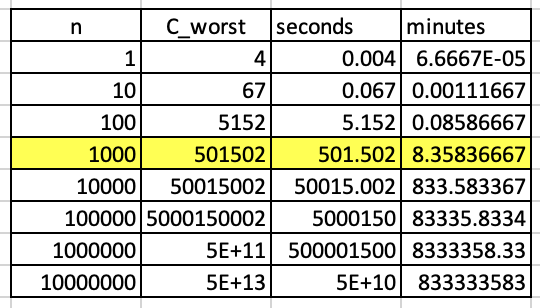
\includegraphics[height=3.5cm]{images/table-2.png}
   \caption{One operation takes 1 ms}
\end{figure}

From the above table, even if we consider that each operation takes 1 millisecond, with an array of length 1000, a computer will theoretically run 501,502 basic operations which take around 8 and a half minutes. A tenfold increase raises the execution time to an extreme 34 hours.
\subsubsection{Limitations}
Thus, a major limitation for the methods in scheduler is that it is inefficient for large arrays.
\\[3pt]
However, as this assignment does not involve testing with large arrays, this limitation is negligible. However for future extensions to this project, it is worth looking into applying more efficient sorting methods than selection. Some of these include insertion, quick-sort and merge sort. 

\section{Test Plan}
Testing was completed using an MSTest project provided by Microsoft in the Visual Studio IDE in the .Net 7.0 framework. The operating system was MacOS Ventura 13.2.1 (22D68) for the M1 Mac-book Pro.
\\[6pt]
To ensure that all aspects of the software system cover functional, non-functional and boundary cases of methods, a comprehensive test plan was designed. 
The plan has been split into three sections that will delve deeper into what was tested each of the three ADTs and why.

\subsection{Testing Job.cs}
The Job class contained the following methods:
\begin{enumerate}
   \item \codeword{IsValidId(uint id)}
   \item \codeword{IsValidExecutionTime(uint executiontime)}
   \item \codeword{IsValidPriority(uint priority)}
   \item \codeword{IsTimeReceived(uint time)}
\end{enumerate}
The goal of each of each of these methods was to return a Boolean value based on whether the parameters they take are valid. It was specified that Id needs to be between 1 and 9 inclusive, and priority needs to be between 1 and 999 inclusive. Additionally, execution time and time received need to simply be greater than 0.
\\[6pt]
For this reason, testing these methods involved providing boundary cases as input and numbers outside the boundary as input. Testing invalid parameter data types was not required as errors are automatically thrown by Visual Studio.

\subsubsection{IsValidId(uint id)}
It was important to test if IsValidId returned true for all values between 1 and 999, and for 1 and 999 themselves. Additionally, it should return false for any values outside the bounds. A summarisation of the results of testing is below and all cases pass, and the method performs as specified. The test data, results and testing code in the \hyperlink{subsubsection.5.1.1}{appendix for IsValidId}.
\\[6pt]
\textbf{Unit testing summarisation}
\begin{figure}[H]
   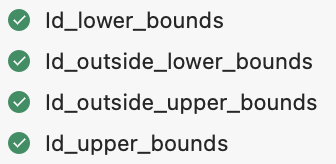
\includegraphics[height=2cm]{images/IsValidId-summary.png}
\end{figure}

\subsubsection{IsValidExecutionTime(uint executiontime)}
Similarly, it was important that IsValidExecutionTime returned true when executionTime was greater than 0, and false for values that were 0 or below. Hence, the values 0 and 1 were used for testing. As summarised below, both tests passed and in the method performs as specified. The test data, results and testing code in the \hyperlink{subsubsection.5.1.3}{appendix for IsValidExecutionTime}.
\\[6pt]
\textbf{Unit testing summarisation}
\begin{figure}[H]
   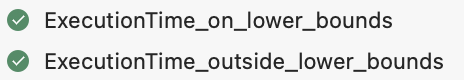
\includegraphics[height=1cm]{images/IsValidExecutionTime-summary.png}
\end{figure}

\subsubsection{IsValidPriority(uint priority)}
In a similar fashion, IsValidPriority was tested for its boundary and functional requirements (requirement is to be between 1 and 9 inclusive). It also passed each test summarised below. The test data, results and testing code in the \hyperlink{subsubsection.5.1.3}{appendix for IsValidPriority}.
\\[6pt]
\textbf{Unit testing summarisation}
\begin{figure}[H]
   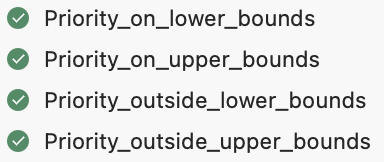
\includegraphics[height=2cm]{images/IsValidPriority-summary.png}
\end{figure}

\subsubsection{IsTimeReceived(uint time)}
Similarly, IsTimeReceived needed to return true when receivedTime was greater than 0 and false for values that were 0 or below. Hence, the values 0 and 1 were used for
testing. As summarised below, both tests passed and in the method performs as specified. The
test data, results and testing code in the \hyperlink{subsubsection.5.1.4}{appendix for IsTimeReceived}.
\\[6pt]
\textbf{Unit testing summarisation}
\begin{figure}[H]
   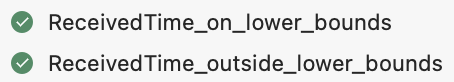
\includegraphics[height=1cm]{images/IsTimeReceived-summary.png}
\end{figure}


\subsection{Testing JobCollection.cs}
The goal of JobCollection is to store and manipulate a collection of jobs. This includes methods for adding and removing a job from a collection, checking if a job is in a collection and finding a job in a collection. It includes an additional method that returns an independent IJob[] array with the same jobs as the collection.

Since these methods all involve collections of jobs, they all use the same job objects, they are common for each test. The jobs used for testing are listed below.
\begin{enumerate}
   \item \codeword{Add(IJob job)}
   \item \codeword{Contains(uint id)}
   \item \codeword{Find(uint id)}
   \item \codeword{Remove(uint id)}
\end{enumerate}

Since these methods all involve collections of jobs, they all use the same \textit{job} objects, they are common for each test. Additionally, each test used a collection with capactity 5, hence an empty \textit{JobCollection} was also used as a public variable. The data used for testing are listed below.
\\[6pt]
\textbf{Common Test Data}
\begin{figure}[H]
   \centering
   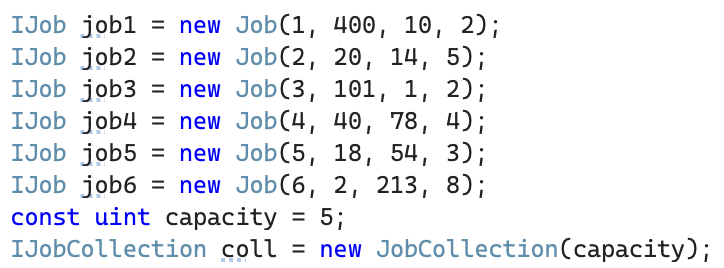
\includegraphics[height=3cm]{images/JobCollection-data.png}
   \caption{IJob objects used throughout testing of JobCollection}
\end{figure}

\subsubsection{Add(IJob job)}
Before testing Contains, Find and Remove. It was important to test if adding jobs to a collection performed as specified.
\\[6pt] 
The first test involved adding a job to an empty array, expecting it to append and return true. Once this was confirmed, the second test was performed and involved adding a job to full array, expecting it to not add the job and return false. The third test involved adding a job that already exists in the collection, expecting it not to add the job and return false. The last test involved adding a null-type job to an empty array, expecting it to not add the job and return false. The data and results are summarised below. The
test data, results and testing code for each test can be found in the \hyperlink{subsubsection.5.2.1}{appendix for Add}.
\\[6pt]
\textbf{Unit testing summarisation}
\begin{figure}[H]
   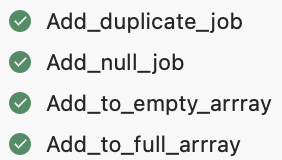
\includegraphics[height=2cm]{images/Add-summary.png}
\end{figure}

\subsubsection{Contains(uint id)}
\textit{Contains} was specified to return true if the supplied \textit{id} matched to a job in a collection and false otherwise. Additionally, if the number of jobs in a collection; \textit{count}, was $0$, the method would return false without looping through the collection. Thus, testing involved checking whether the correct boolean values were returned if a job wasn't in a collection, was in a collection, and if a collection had no jobs to begin with. The summary below shows that each of these tests passed and test specific data, results and code can be found in the \hyperlink{subsubsection.5.2.2}{appendix for Contains}
\\[6pt]
It is worth noting that testing the scenario where the capacity is one could have been useful to safeguard against incorrect ranges in a \codeword{for} loop, however, a \codeword{while} loop was used thus making this test unnecessary.
\\[6pt]
\textbf{Unit testing summarisation}
\begin{figure}[H]
   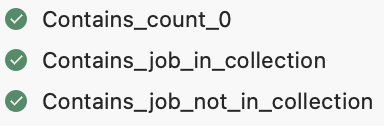
\includegraphics[height=1.5cm]{images/Contains-summary.png}
\end{figure}

\subsubsection{Find(uint id)}
\textit{Find} was specified to return null if the supplied \textit{id} didn't match with any jobs in a collection and returning the job object if it did match. Additionally, it used \textit{Contains} to first check if the collection contained a job with the supplied \textit{id}. Testing however didn't check if this line ran as the \textit{Contains} method was already tested to perform as specified before \textit{Find}. Thus testing only checked whether \textit{null} or a correct \textit{job} was returned depending on the supplied id. The below summary shows that both tests passed. Test specific data, results and code can be found in the \hyperlink{subsubsection.5.2.3}{appendix for Find}.
\\[6pt]
\textbf{Unit testing summarisation}
\begin{figure}[H]
   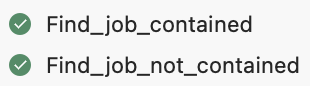
\includegraphics[height=1cm]{images/Find-summary.png}
\end{figure}

\subsubsection{Remove(uint id)}
\textit{Remove} was specified to remove a job in a collection that matched the specified \textit{id}, decrease the \textit{count} by 1 and then return true. If the job doesn't exist, then simply return false. Thus it was tested whether the method returns false when not removed and \textit{count} remains unchanged. It was also tested that when \textit{Remove} removes a job successfully, the method returns true, the count decrements by one, and the removed job can no longer be found in the array. The summarisation of results below shows that both tests passed and \textit{Remove} operates as specified. Test data, results and code can be found in the \hyperlink{subsubsection.5.2.4}{appendix for Remove}.
\\[6pt]
\textbf{Unit testing summarisation}
\begin{figure}[H]
   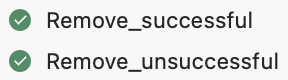
\includegraphics[height=1cm]{images/Remove-summary.png}
\end{figure}

\subsubsection{ToArray}
\textit{ToArray} was specified to simply return an independent array with the same jobs in a collection. It was important to check that ToArray returned the same jobs in the same order, thus this was the only test completed.

The summarisation of results below shows that both tests passed and \textit{Remove} operates as specified. Test data, results and code can be found in the \hyperlink{subsubsection.5.2.5}{appendix for ToArray}.
\\[6pt]
\textbf{Unit testing summarisation}
\begin{figure}[H]
   
\includegraphics[height=0.5cm]{images/ToArray-summary.png}
\end{figure}

\subsection{Testing Scheduler.cs}
\subsubsection{Unit testing methodology}
As mentioned in the beginning of the report, the three alogorithms designed were \codeword{FirstComeFirstServed}, \codeword{ShortestJobFirst} and \codeword{Priority}. Each method was tested data under the same set of conditions, however used different job objects as the test data.
\\[3pt] 
It is important to note that when the phrase \textbf{tested parameter} is mentioned, this refers to either, \textit{receivedTime}, \textit{executionTime} or \textit{priority}, depending on whether \codeword{FirstComeFirstServed}, \codeword{ShortestJobFirst} and \codeword{Priority} are being tested respectively. 
\\[6pt]
Testing worked by creating an array of \textit{uint} values called \textit{expected} which has the expected order of the \textit{tested parameter} for each job. An \textit{actual} array of the same type was created which contains the \textit{tested parameter} for each job sorted using the relevant method. 
\\[3pt]
These were then compared using \codeword{bool assertion = Enumerable.SequenceEqual(actual, expected)} which would return true if each value in the two arrays was the same, i.e., the \textit{FirstComeFirstServed} method correctly sorted the \textit{JobCollection}, and false otherwise. Since unit testing was used, 

\codeword{Assert.IsTrue(assertion)}, was added to the testing method.
\\[3pt]
\subsubsection{Testing methods}
One condition was testing if a collection was sorted correctly when all jobs had unique parameters for the \textit{tested parameter}. For example, \textit{Priority} would be tested to sort a collection with jobs that all had unique \textit{priority} parameters. The goal of this test was to ensure that the order of a sorted collection was correct. 
\\[3pt]
The next condition also used unique parameters for the \textit{tested parameter}, but used a partially full collection. This was important to ensure that the sorting methods would return arrays with null values at the end and wouldn't throw exceptions when encountering null objects.
\\[6pt]
Thus, these conditions were tested using the methods; 

\codeword{unique_jobs_in_a_full_collection} and \codeword{unique_jobs_in_a_partial_collection}.
\\[10pt]
Additionally, in order to test whether multiple computing jobs that have the same \textit{tested parameter}, are executed in any order, two other methods used collections that had some jobs with the same \textit{tested parameter}. 
\\[3pt]
Thus two other methods were used for testing. These were \codeword{common_jobs_in_a_full_collection} and \codeword{common_jobs_in_a_partial_collection}.
\\[10pt]
The last test involved sorting a collection with a single job. This was important to ensure that the methods would not use indexes out of the range of the collection. This test was named \codeword{collection_capacity_one}.
\\[3pt]
It was deemed unnecessary to supply an empty collection to a sorting method as the methods are based on the $Count$ variable; the number of jobs, rather than $Capacity$. Hence this was not tested.
\\[10pt]
Thus the list of test methods can be summarised below.
\begin{enumerate}
   \item \codeword{unique_jobs_in_a_full_collection}
   \item \codeword{unique_jobs_in_a_partial_collection}
   \item \codeword{common_jobs_in_a_full_collection}
   \item \codeword{common_jobs_in_a_partial_collection}
   \item \codeword{collection_capacity_one}
\end{enumerate}

\subsubsection{FirstComeFirstServed}
Each test used the same \textit{job} objects, and a \textit{JobCollection} with capacity $7$. Note that \textit{priority} and \textit{executionTime} are held constant as they are not relevant to the \textit{FirstComeFirstServed} sorting algorithm.
\\[6pt]
\textbf{Common Test Data}
\begin{figure}[H]
   \centering
   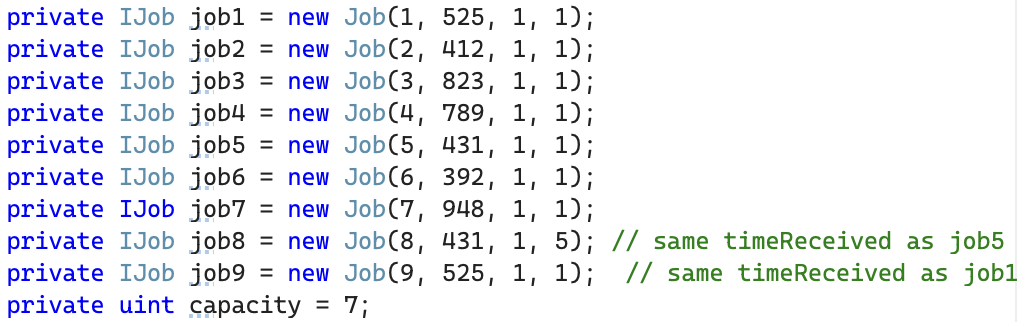
\includegraphics[height=4cm]{images/FCFS-data.png}
   \caption{IJob objects used throughout testing of FirstComeFirstServed}
\end{figure}
While actual unit testing was done differently, the test data, expected results, and test results are simply displayed as lists of jobs. The exact \textit{Jobs} used did differ for each test and this input data along with expected and resulting data can be found in the \hyperlink{subsubsection.5.3.1}{appendix for FirstComeFirstServed}.
\\[3pt]
From the below summary of tests it can be seen that each test passed and thus \textit{FirstComeFirstServed} was verified to perform as specified.
\pagebreak

\textbf{Unit testing summarisation}
\begin{figure}[H]
   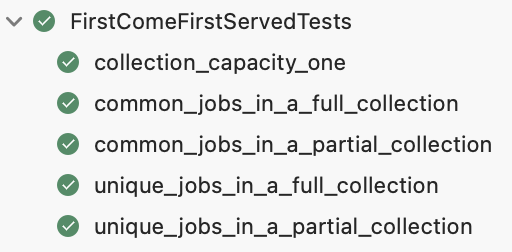
\includegraphics[height=3.5cm]{images/FCFS-summary.png}
\end{figure}

\subsubsection{ShortestJobFirst}
Similarly to \textit{FirstComeFirstServed}, methods for testing \textit{ShortestJobFirst} used the same \textit{job} objects, and a \textit{JobCollection} with capacity $7$. Note that \textit{priority} and \textit{receivedTime} are held constant as they are not relevant to the \textit{ShortestJobFirst} sorting.
\\[6pt]
\textbf{Common Test Data}
\begin{figure}[H]
   \centering
   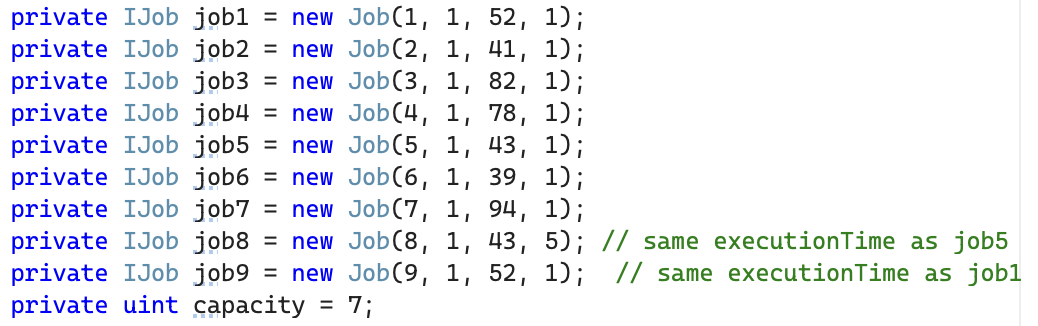
\includegraphics[height=4cm]{images/SJF-data.png}
   \caption{IJob objects used throughout testing of ShortestJobFirst}
\end{figure}
While actual unit testing was done differently, the test data, expected results, and test results are simply displayed as lists of jobs. The exact \textit{Jobs} used did differ for each test and this input data along with expected and resulting data can be found in the \hyperlink{subsubsection.5.3.1}{appendix for ShortestJobFirst}.
\\[3pt]
From the below summary of tests it can be seen that each test passed and thus \textit{ShortestJobFirst} was verified to perform as specified.

\textbf{Unit testing summarisation}
\begin{figure}[H]
   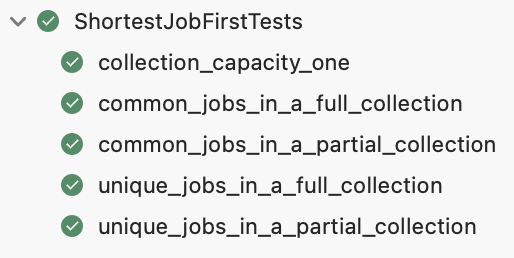
\includegraphics[height=3.5cm]{images/SJF-summary.png}
\end{figure}

\pagebreak
\subsubsection{Priority}
Similarly to the other two sorting algorithms, testing methods for \textit{Priority} used the same \textit{job} objects, and a \textit{JobCollection} with capacity $7$. Note that \textit{executionTime} and \textit{receivedTime} are held constant as they are not relevant to the \textit{ShortestJobFirst} sorting.
\textbf{Common Test Data}
\begin{figure}[H]
   \centering
   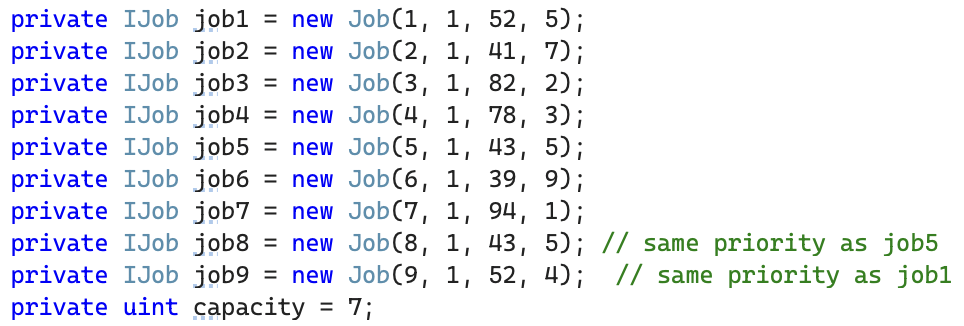
\includegraphics[height=4cm]{images/Priority-data.png}
   \caption{IJob objects used throughout testing of Priority}
\end{figure}
While actual unit testing was done differently, the test data, expected results, and test results are simply displayed as lists of jobs. The exact \textit{Jobs} used did differ for each test and this input data along with expected and resulting data can be found in the \hyperlink{subsubsection.5.3.1}{appendix for Priority}.
\\[3pt]
From the below summary of tests it can be seen that each test passed and thus \textit{Priority} was verified to perform as specified.
\\[6pt]
\textbf{Unit testing summarisation}
\begin{figure}[H]
   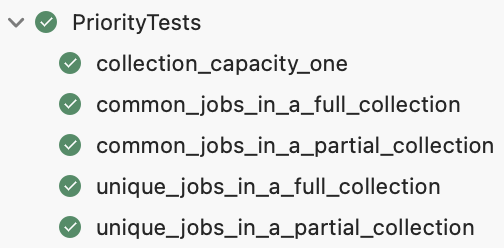
\includegraphics[height=3.5cm]{images/Priority-summary.png}
\end{figure}

\section{References}
Levitin, A. (2012). Introduction to The Design \& Analysis of Algorithms. In A. Levitin, 

Introduction to The Design \&Analysis of Algorithms (Vol. 3). New Jersey, 

United States of America: Pearson Education.
\pagebreak

\section{Appendix}
\subsection{Job ADT test data, results and code}
\subsubsection{IsValidId{()}}
\begin{figure}[H]
   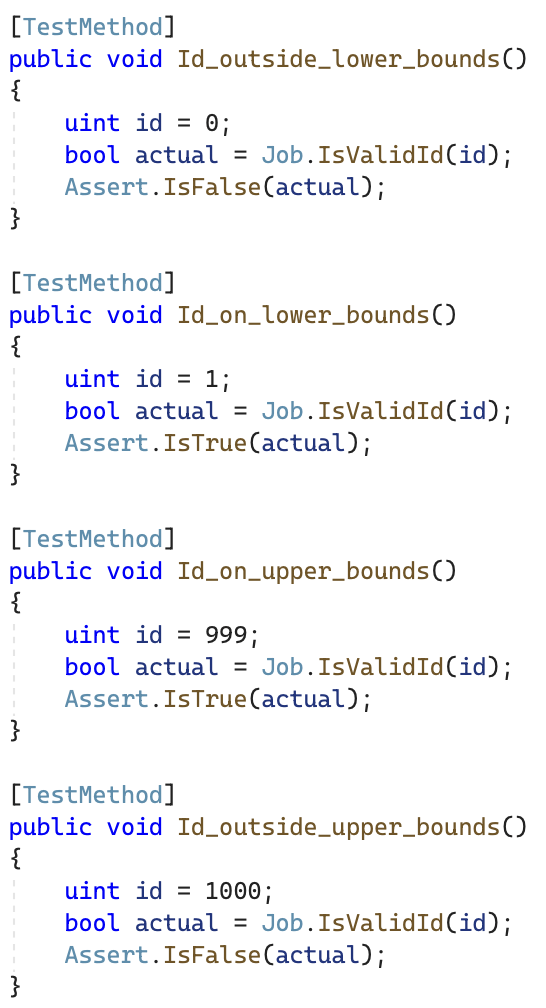
\includegraphics[height=11cm]{images/IsValidId.png}
   \caption{Unit testing for IsValidId}
\end{figure}

\subsubsection{IsValidExecutionTime{()}}
\begin{figure}[H]
   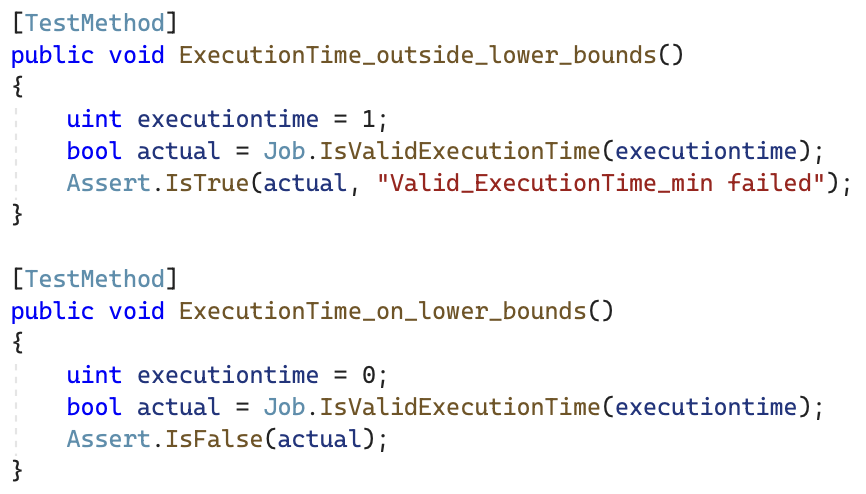
\includegraphics[height=5cm]{images/IsValidExecutionTime.png}
   \caption{Unit testing for IsValidExecutionTime}   
\end{figure}

\subsubsection{IsValidPriority{()}}
\begin{figure}[H]
   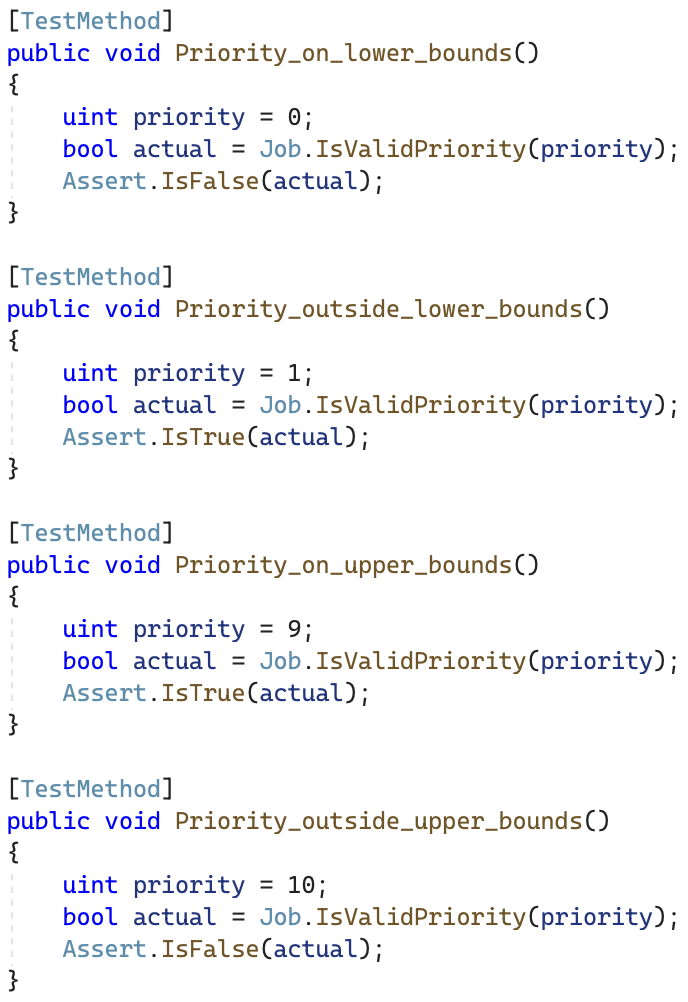
\includegraphics[height=11cm]{images/IsValidPriority.png}
   \caption{Unit testing for IsValidPriority}
\end{figure}

\subsubsection{IsTimeReceived{()}}
\begin{figure}[H]
   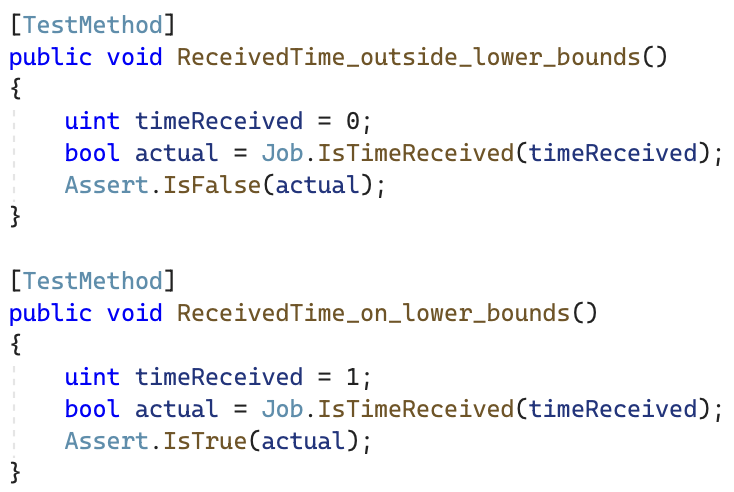
\includegraphics[height=5cm]{images/IsTimeReceived.png}
   \caption{Unit testing for IsTimeReceived}
\end{figure}


\subsection{JobCollection ADT test data, results and code}
\subsubsection{Add{()}}
\begin{figure}[H]
   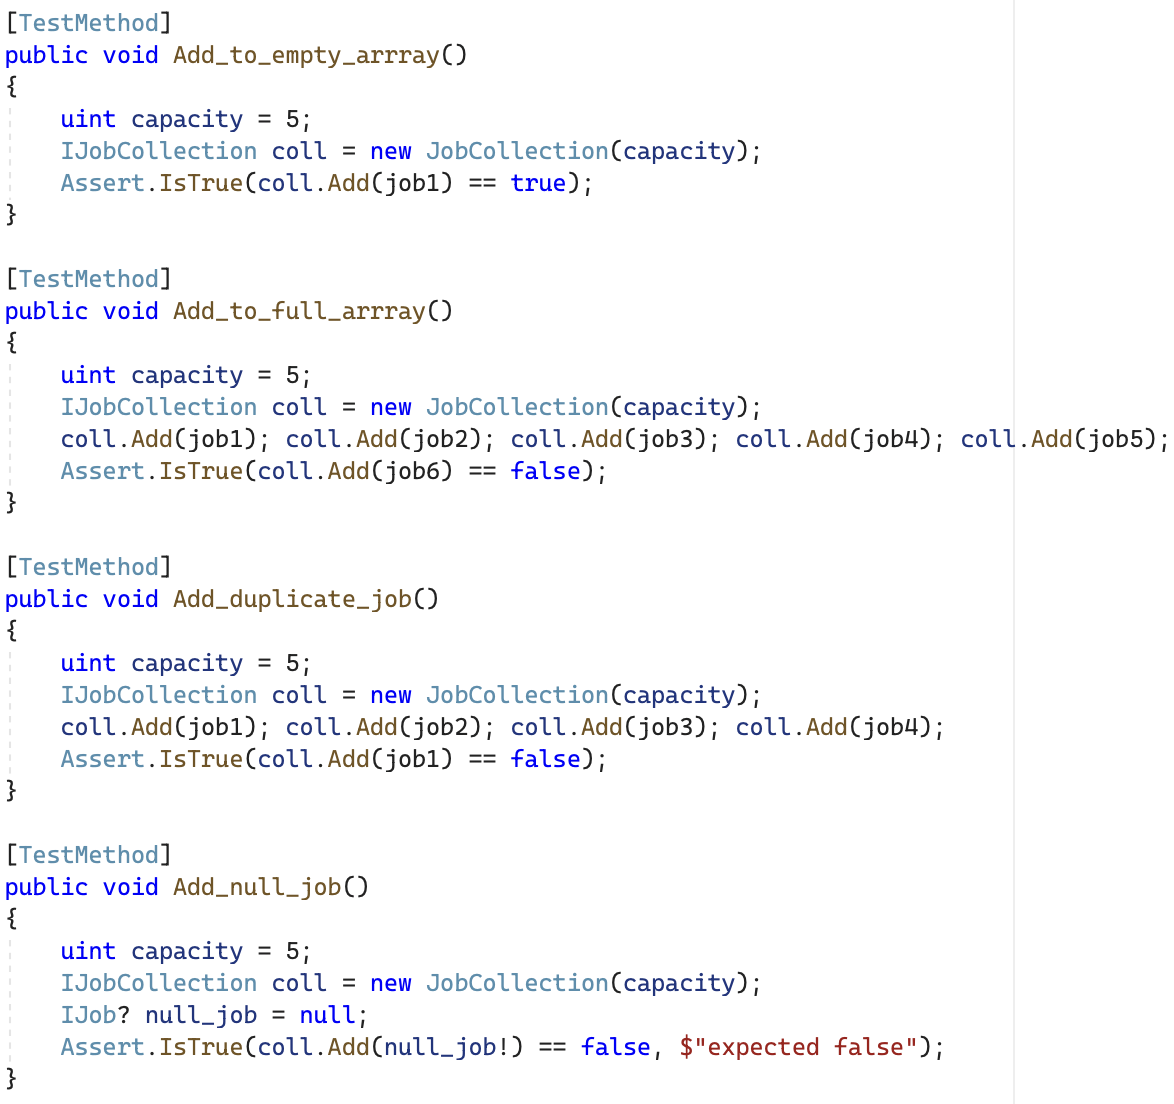
\includegraphics[height=11cm]{images/Add.png}
   \caption{Unit testing for Add}
\end{figure}

\subsubsection{Contains{()}}
\begin{figure}[H]
   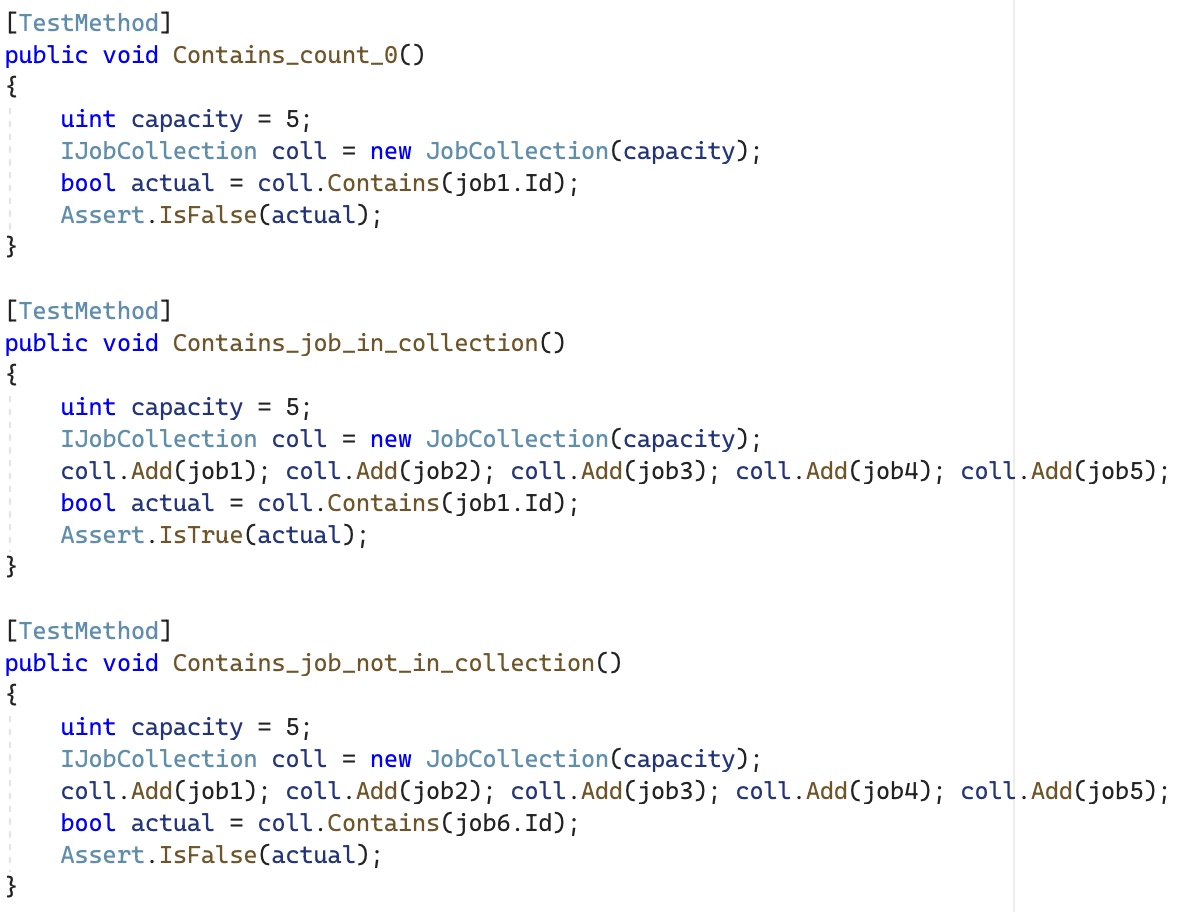
\includegraphics[height=9cm]{images/Contains.png}
   \caption{Unit testing for Contains}
\end{figure}

\subsubsection{Find{()}}
\begin{figure}[H]
   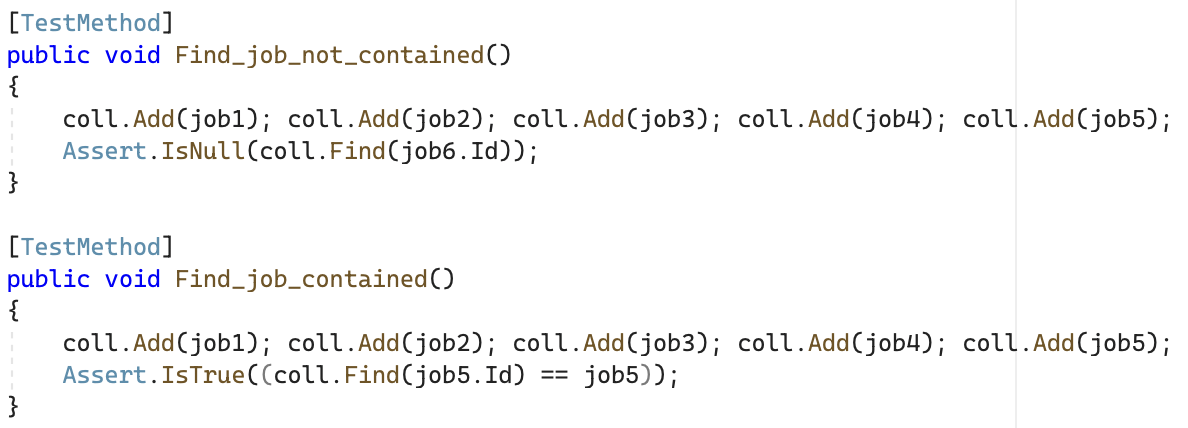
\includegraphics[height=4.5cm]{images/Find.png}
   \caption{Unit testing for Find}
\end{figure}

\subsubsection{Remove{()}}
\begin{figure}[H]
   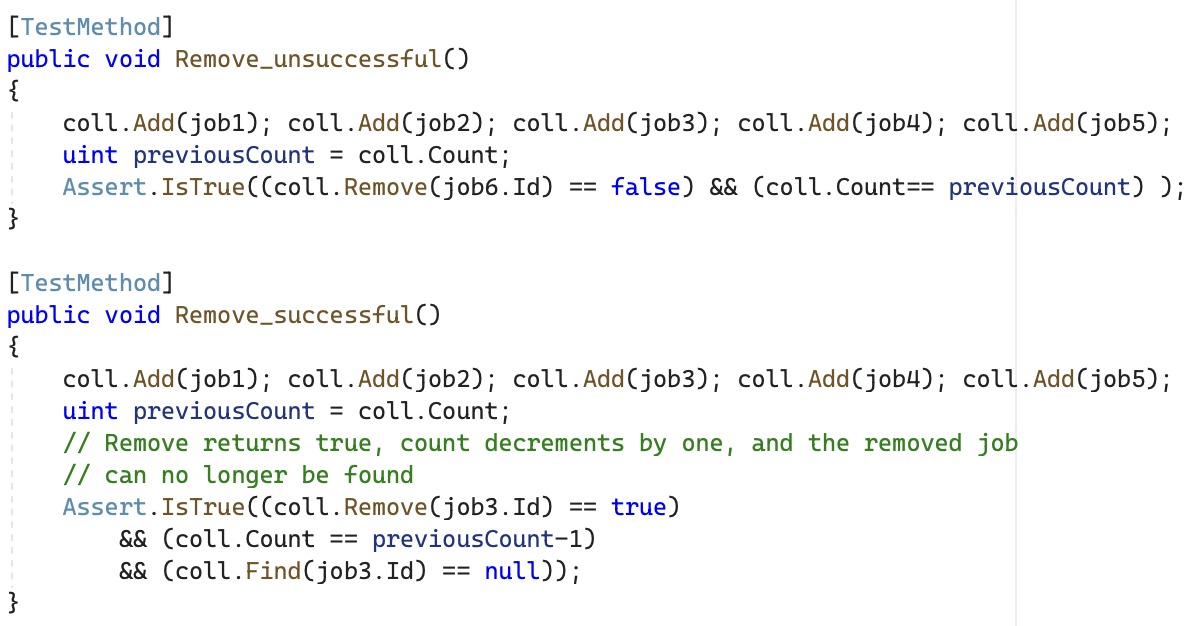
\includegraphics[height=6cm]{images/Remove.png}
   \caption{Unit testing for Remove}
\end{figure}

\subsubsection{ToArray{()}}
\begin{figure}[H]
   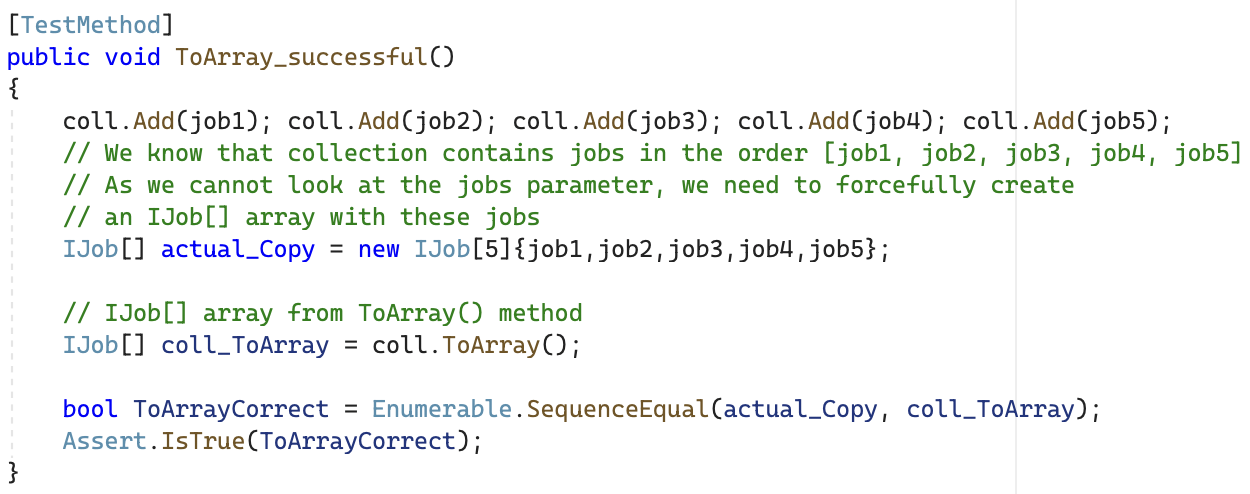
\includegraphics[height=5cm]{images/ToArray.png}
   \caption{Unit testing for ToArray}
\end{figure}

\subsection{Scheduler ADT test data, results and code}

\subsubsection{FirstComeFirstServed}
\begin{figure}[H]
   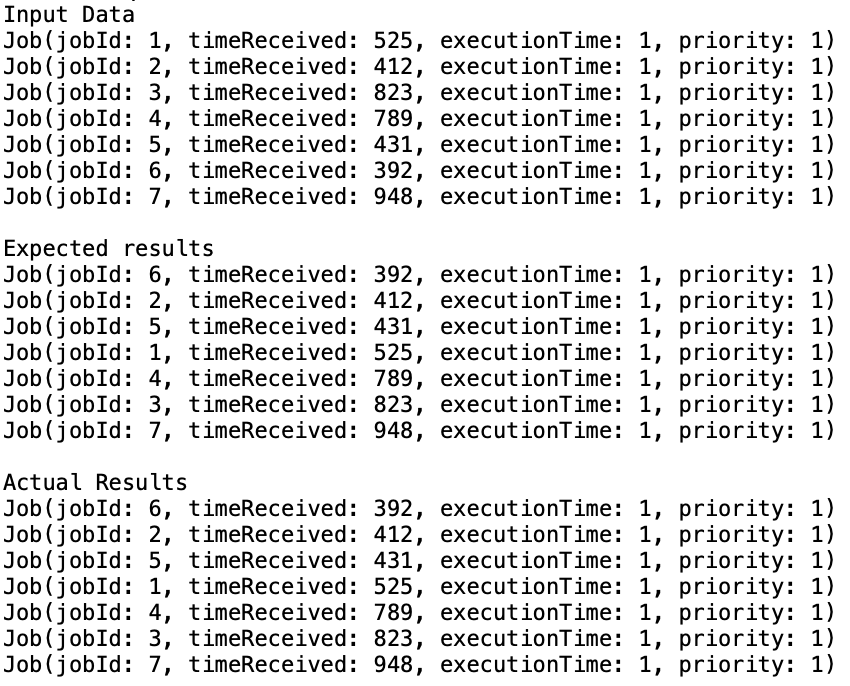
\includegraphics[height=8.2cm]{images/FCFS-unique_jobs_in_a_full_collection.png}
   \caption{Unit testing for unique\_jobs\_in\_a\_full\_collection}
\end{figure}

\begin{figure}[H]
   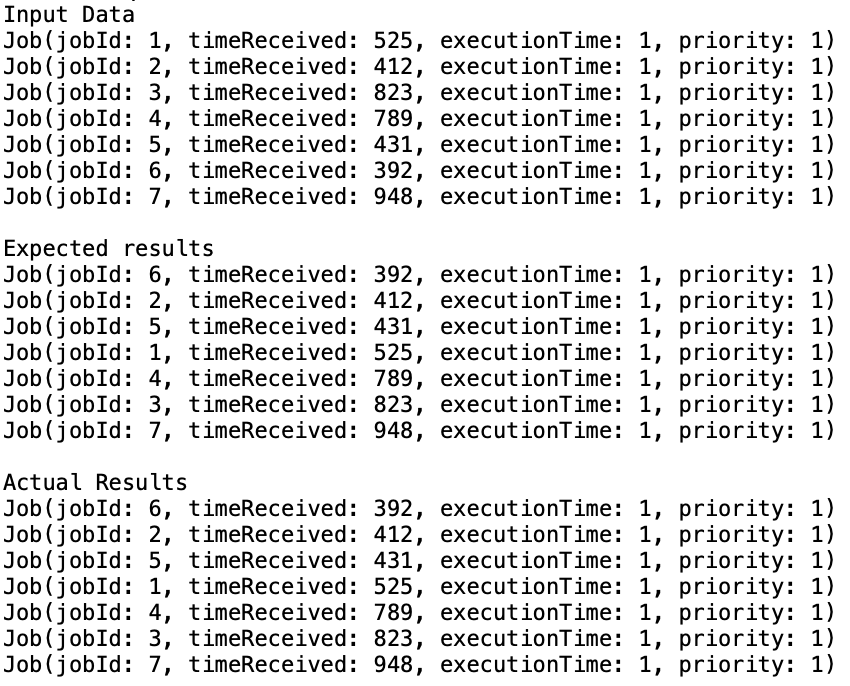
\includegraphics[height=8.2cm]{images/FCFS-unique_jobs_in_a_full_collection.png}
   \caption{Unit testing for unique\_jobs\_in\_a\_partial\_collection}
\end{figure}

\begin{figure}[H]
   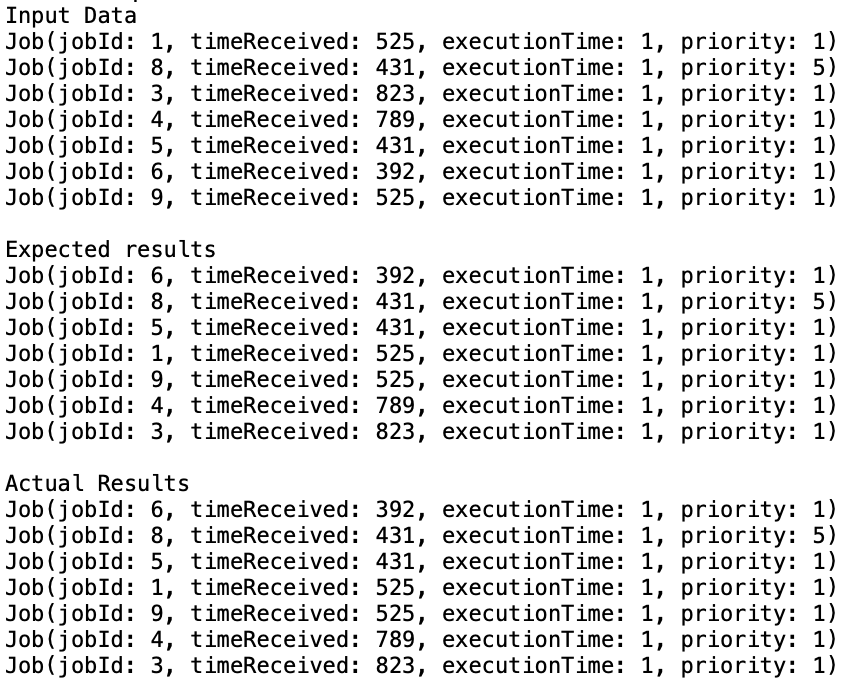
\includegraphics[height=8.2cm]{images/FCFS-common_jobs_in_a_full_collection.png}
   \caption{Unit testing for common\_jobs\_in\_a\_full\_collection}
\end{figure}

\begin{figure}[H]
   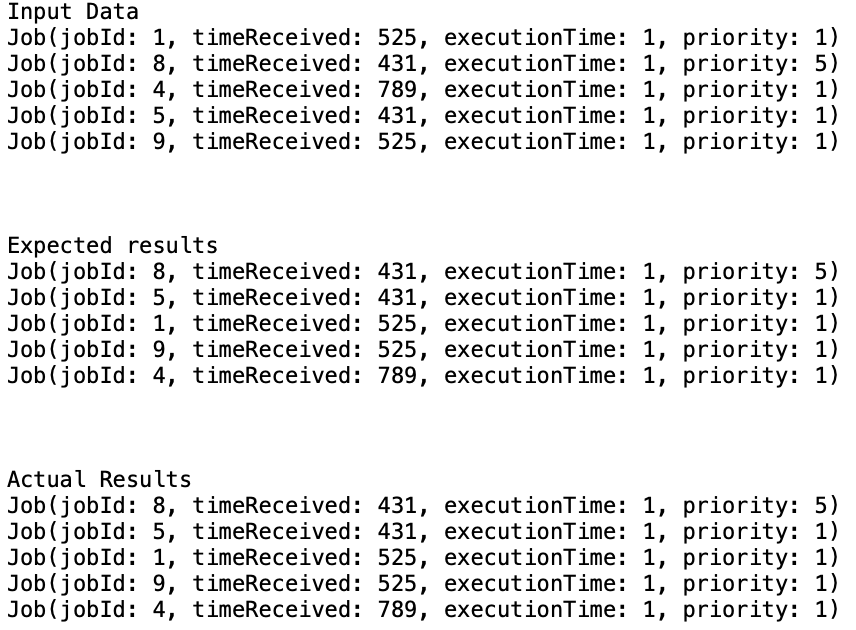
\includegraphics[height=8.2cm]{images/FCFS-common_jobs_in_a_partial_collection.png}
   \caption{Unit testing for common\_jobs\_in\_a\_partial\_collection}
\end{figure}

\begin{figure}[H]
   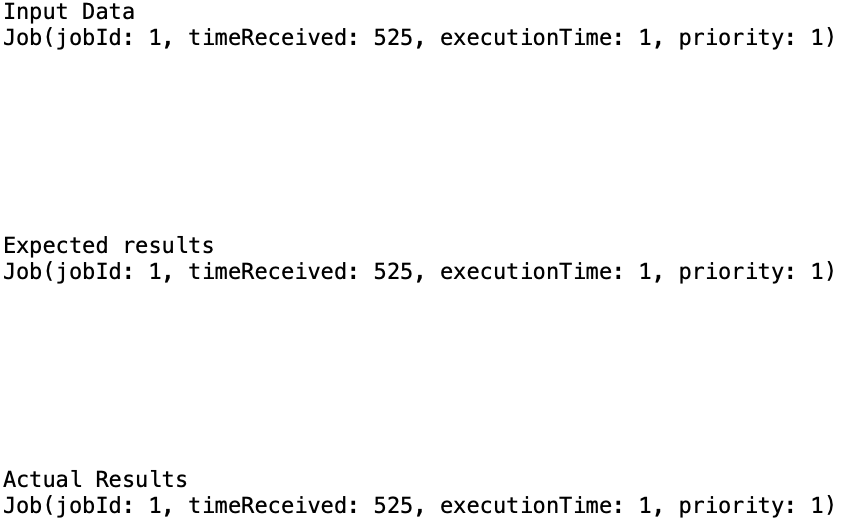
\includegraphics[height=6cm]{images/FCFS-collection_capacity_one.png}
   \caption{Unit testing for collection\_capacity\_one}
\end{figure}

\subsubsection{Shortest Job First}
\begin{figure}[H]
   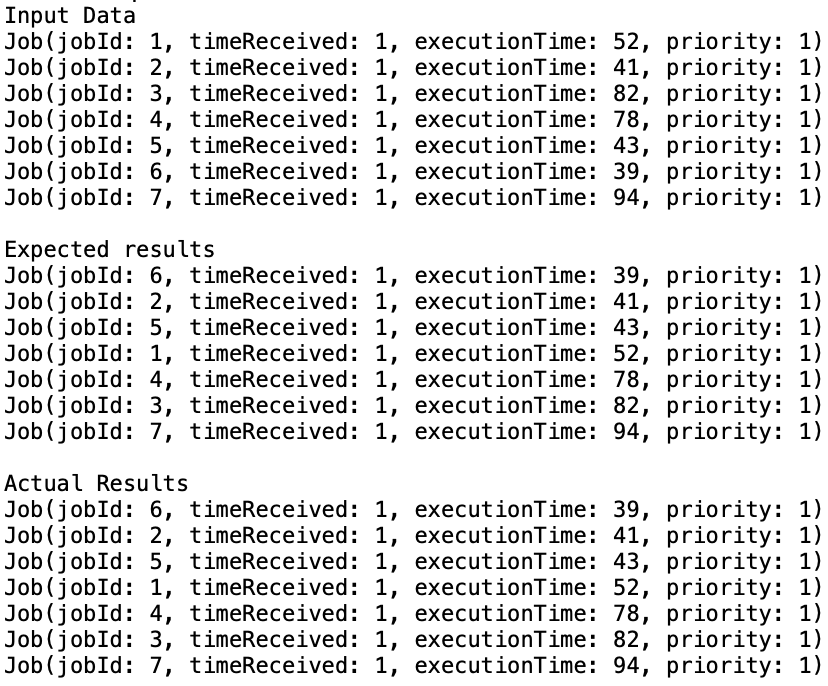
\includegraphics[height=8.2cm]{images/SJF-unique_jobs_in_a_full_collection.png}
   \caption{Unit testing for unique\_jobs\_in\_a\_full\_collection}
\end{figure}

\begin{figure}[H]
   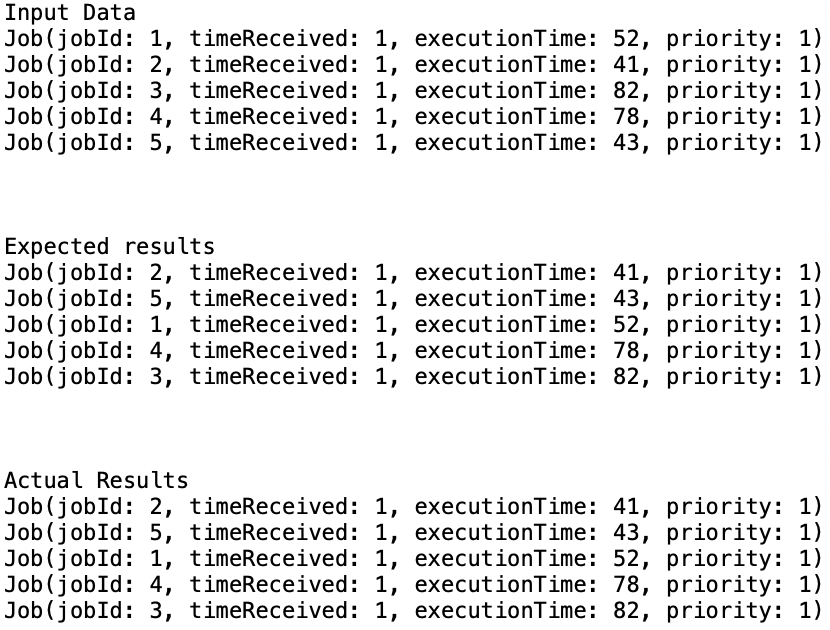
\includegraphics[height=9cm]{images/SJF-unique_jobs_in_a_partial_collection.png}
   \caption{Unit testing for unique\_jobs\_in\_a\_partial\_collection}
\end{figure}

\begin{figure}[H]
   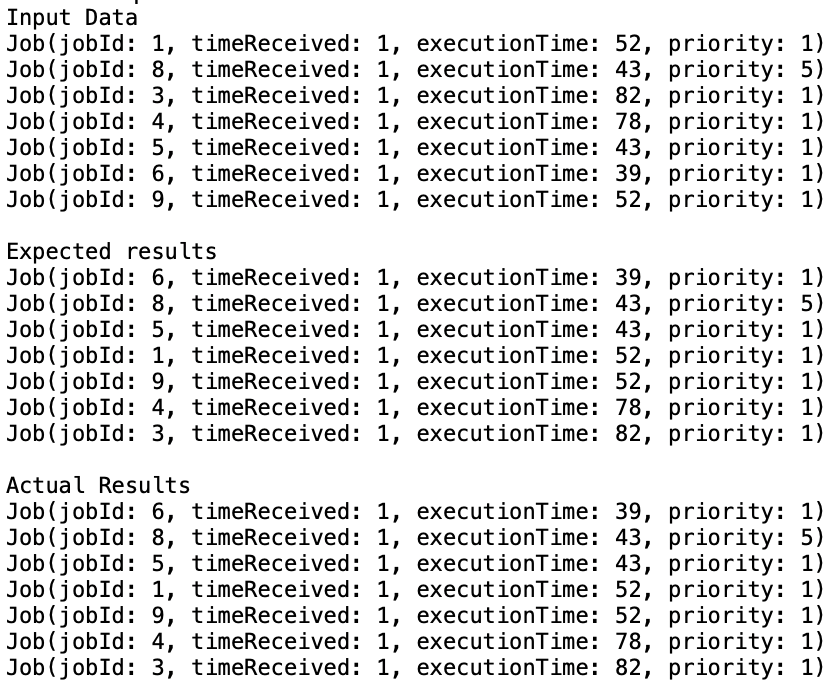
\includegraphics[height=9cm]{images/SJF-common_jobs_in_a_full_collection.png}
   \caption{Unit testing for common\_jobs\_in\_a\_full\_collection}
\end{figure}

\begin{figure}[H]
   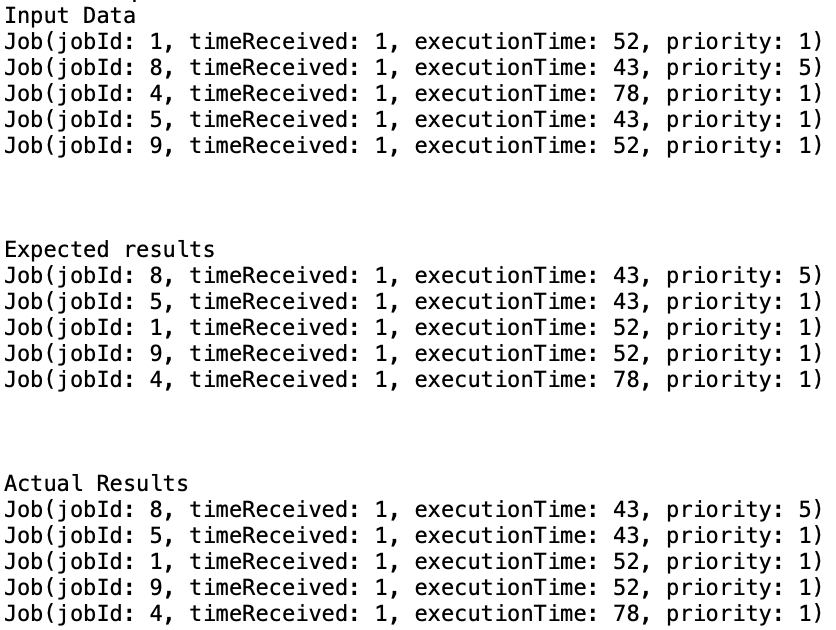
\includegraphics[height=8.2cm]{images/SJF-common_jobs_in_a_partial_collection.png}
   \caption{Unit testing for common\_jobs\_in\_a\_partial\_collection}
\end{figure}

\begin{figure}[H]
   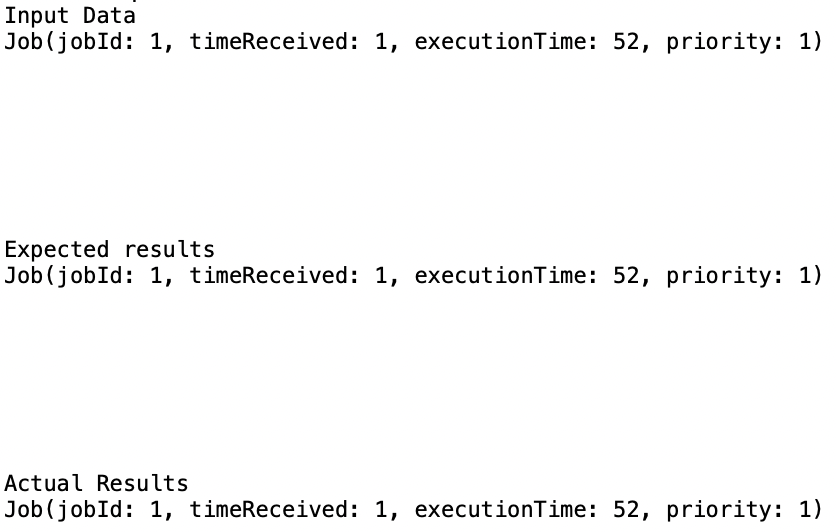
\includegraphics[height=6cm]{images/SJF-collection_capacity_one.png}
   \caption{Unit testing for collection\_capacity\_one}
\end{figure}

\subsubsection{Priority}
\begin{figure}[H]
   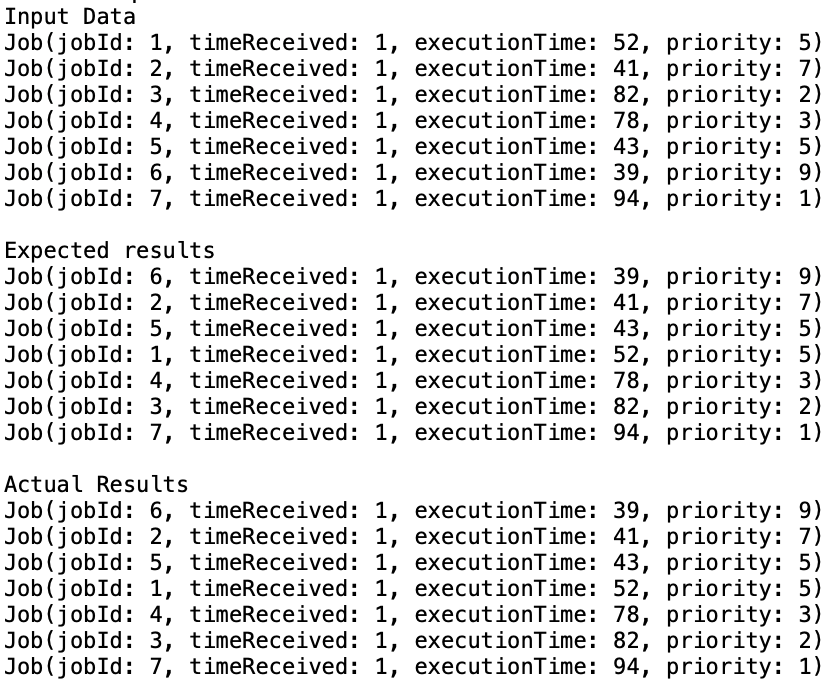
\includegraphics[height=8.2cm]{images/Priority-unique_jobs_in_a_full_collection.png}
   \caption{Unit testing for unique\_jobs\_in\_a\_full\_collection}
\end{figure}

\begin{figure}[H]
   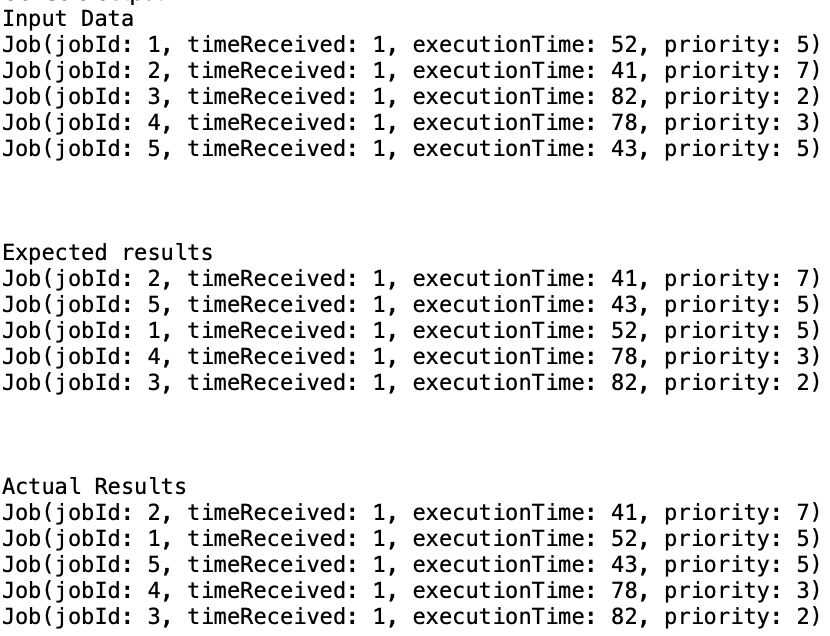
\includegraphics[height=9cm]{images/Priority-unique_jobs_in_a_partial_collection.png}
   \caption{Unit testing for unique\_jobs\_in\_a\_partial\_collection}
\end{figure}

\begin{figure}[H]
   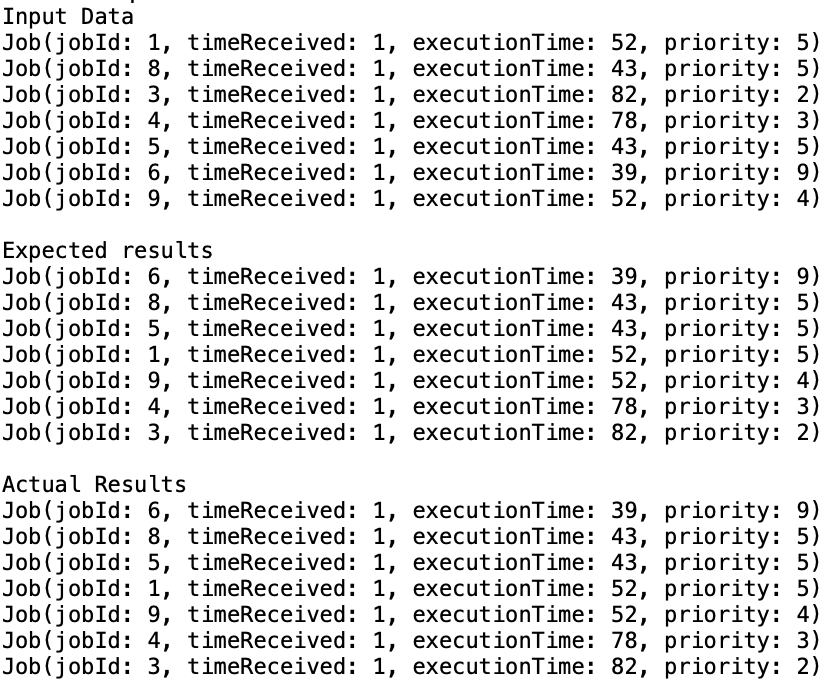
\includegraphics[height=9cm]{images/Priority-common_jobs_in_a_full_collection.png}
   \caption{Unit testing for common\_jobs\_in\_a\_full\_collection}
\end{figure}

\begin{figure}[H]
   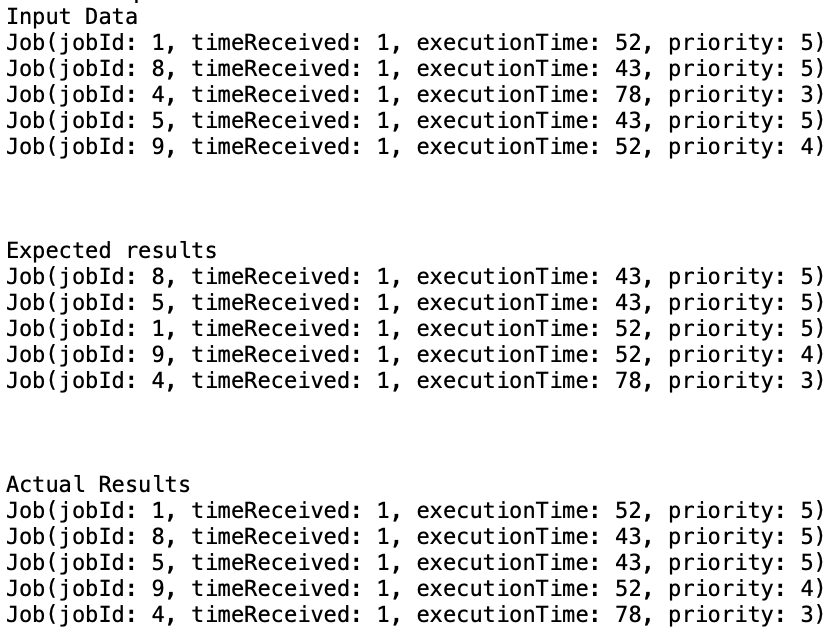
\includegraphics[height=8.2cm]{images/Priority-common_jobs_in_a_partial_collection.png}
   \caption{Unit testing for common\_jobs\_in\_a\_partial\_collection}
\end{figure}

\begin{figure}[H]
   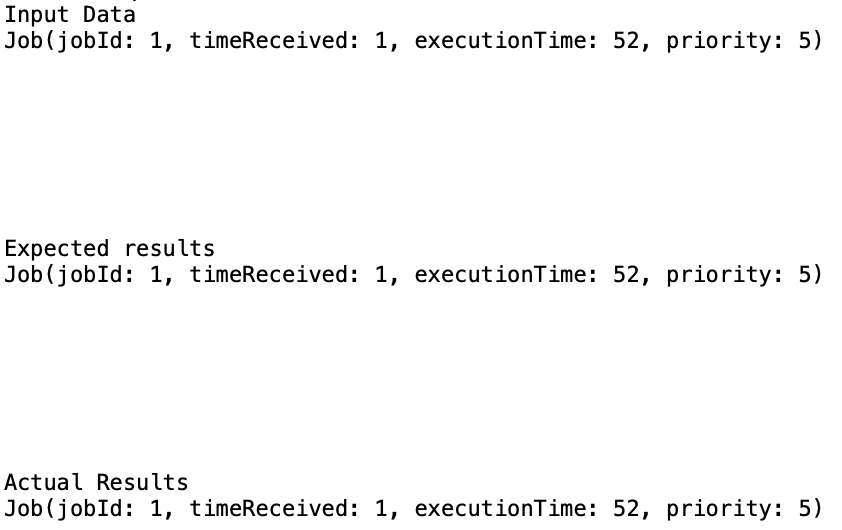
\includegraphics[height=6cm]{images/Priority-collection_capacity_one.png}
   \caption{Unit testing for collection\_capacity\_one}
\end{figure}

\end{document}